% DOCUMENT CLASS %
\documentclass[a4paper, 12pt]{article}   % for A4 Paper, 12pt fontsize.
\setcounter{tocdepth}{4}
\setcounter{secnumdepth}{3}

% PACKAGES%
\usepackage{amsfonts}   % For a basic mathfont (many will be replaced by stix)
\usepackage{amsmath}    % For basic math symbols
%\usepackage{bbm}        % For \mathbbm (better version of \mathbb)
\usepackage{mathrsfs}   % For \mathscr
\usepackage{hyperref}   % For footnotes
\usepackage{csquotes}   % For \textquote{}
\usepackage{IEEEtrantools}  % For better alignments
\usepackage{tikz}   % For a macro
\usepackage{listings} % For code
\usepackage{xcolor}   % For ... code
\usepackage[stretch=40]{microtype}
\usepackage{enumitem}
\usepackage{geometry}
\usepackage[color=gray]{todonotes}

% Language
\usepackage[english]{babel}

% If needed
\usepackage[nohyperlinks,smaller]{acronym}

% For tests
\usepackage{lipsum}

%%% ENVIRONMENTS %%%
\usepackage{amsthm}
\usepackage[nameinlink]{cleveref}

% Definition environment
\theoremstyle{definition}
\newtheorem{definition}{Definition}[section]
% Configure reference name
\crefname{definition}{Definition}{Definitions}

\theoremstyle{definition}
\newtheorem{exercise}{Exercise}[section]
\crefname{exercise}{Exercise}{Exercises}

\theoremstyle{definition}
\newtheorem{algorithm}{Algorithm}%[section]
\crefname{algorithm}{Algorithm}{Algorithms}

\theoremstyle{theorem}
\newtheorem{theorem}{Theorem}%[section]
\crefname{theorem}{Theorem}{Theorems}
%%%

%%% FONT CONFIGURATION %%%
\usepackage{fontspec}

% Updated version of Crimson Text
\setmainfont{Cochineal}
\setmonofont{Cascadia Code}[Scale=0.8]
\usepackage[cochineal]{newtxmath} % To use Cochineal as a Math Font
%%%

% MAKE DESCRIPTION ENVIRONMENTS HAVE ITALICIZED ITEMS %
\renewcommand{\descriptionlabel}[1]{\hspace{\labelsep}\textit{#1}}

% SETS %
\newcommand*{\R}{\mathbb R}    % Set of real numbers
\newcommand*{\N}{\mathbb N}    % Set of natural numbers
\newcommand*{\Z}{\mathbb Z}    % Set of integers
\newcommand*{\Q}{\mathbb Q}    % Set of rational numbers

% BASIC CONFIGURATION %
\pagestyle{plain}
\allowdisplaybreaks

% CODE %
\definecolor{codepurple}{HTML}{7f0055}
\definecolor{comment}{RGB}{0,128,0}
\definecolor{number}{RGB}{9,136,90}
\definecolor{string}{RGB}{163,21,21}

% Things that are the same in all styles
\lstdefinestyle{basic}{
    basicstyle=\ttfamily\footnotesize,
    breakatwhitespace=false,
    breaklines=true,
    frame=leftline,
    keepspaces=true,
    numbers=left,
    firstnumber=1,
    numbersep=5pt,
    showspaces=false,
    showstringspaces=false,
    showtabs=false,
    tabsize=2,
    commentstyle=\itshape\color{comment},
    stringstyle=\color{string},
    keywordstyle=\bfseries\color{codepurple},
    texcl=true,
    mathescape=true
}

\lstdefinestyle{default}{
    style=basic,
    language=c,
}

\lstset{style=default}

\title{Internet of Things and Wireless Networks}
\date{Summer Term 2026}
\author{Henri Heyden \\%
    \small stu240825 \\%
    \and%
    Parham Razaghian \\%
    \small stu258323%
}


\begin{document}
\maketitle

\section{Project}
In our project we looked at the following tasks.

\paragraph{Task 1: 5 Points}
Setup one device which relays RSSIs of foreign advertisements to a general purpose computer to convert to distance.

\paragraph{Task 2: 10 Points}
Setup three devices which relay the RSSIs of one device to a general purpose computer and triangulate the position.

\paragraph{Task 3: 15 Points}
Calculate a dynamic visualization on the general purpose device to track the movement of the user device.

\subsection{Solution for Task 1}
For the first task we programmed firmware for one ESP32 chip, which continuously scans for BLE traffic.
If a message is received, the following payload is redirected via a central-peripheral connection to my laptop.
\begin{lstlisting}
typedef struct __packed
{
    uint8_t nodeID;      // Our node ID. Either 1, 2, or 3.
    int64_t timestamp;   // Used by the peripheral to calculate accurate positioning.
    int8_t rssi;         // RSSI of the traffic we received.
    bt_addr_le_t sender; // Address of the device which sent the traffic.
} message_t;
\end{lstlisting}
The laptop then logs the content of all messages received to a file.
We then use another python script to evaluate the data and convert it to a distance.
The distance calculation is based on the following method.
\begin{IEEEeqnarray*}{r'c'l}
    d & = & 10 ^ {\frac{R_0 - R}{10 N}}
\end{IEEEeqnarray*}
Here, \(R_0\) is the RSSI at distance one meter, \(R\) is the RSSI, and \(N \in [2, 4]\) is an environmental parameter.
This meant, that to measure the distance to a certain device, we needed to calibrate the equipment, such that the \(R_0\) parameter is known.

This is of course very tedious, as any individual sender-receiver pair would mean a different \(R_0\), which is why we used my headphones and one specific ESP32 to calibrate the system and record data.
See \autoref{fig:1} for an example plot.

\begin{figure}[h]
    \centering
    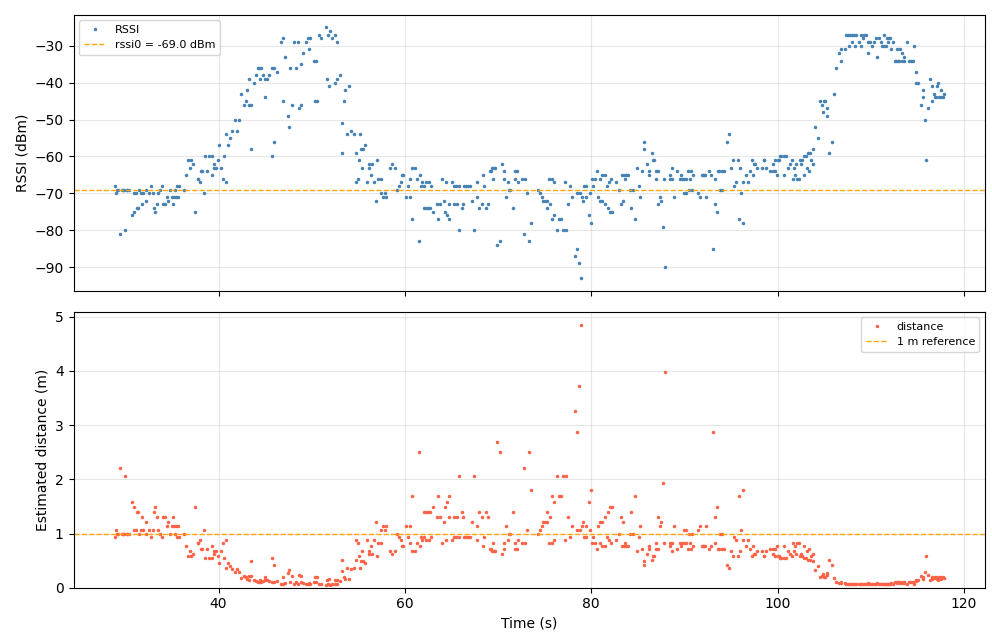
\includegraphics[width=\textwidth]{../code/peripheral/plots/estimated_distance.png}
    \caption{Distance and RSSI between a node and my Bluetooth headphones in pairing mode calculated using the first method.}
    \label{fig:1}
\end{figure}

As seen in \autoref{fig:1}, once we go beyond one meter, the RSSI becomes pretty noisy.
In reality I went from one meter to zero meters and then increased my distance by one meter every time and waited a bit, and finally returned to zero meters at the end.
But distances between zero and one meter are pretty exact.
Thus, a system like this, ideally with some passing mean or other denoising filter, can be used for proximity detection.

\subsection{Solution for Task 2}
For the second task we deployed three nodes in an approximately equidistant triangle with the same firmware, but with different node ids.
We then stood before a decision on how to triangulate the position of a device, based on RSSIs of three devices.
There were three possible approaches.

\subsubsection{Direct Triangulation}
We could use the method for task 1 to converts RSSIs to distances, and triangulate using Barycentric coordinates.
This would mean calibrating each device/node pair for the devices we want to track, and the three nodes, as it would need RSSIs at distance one meter.
All this overhead prompted us to look a bit further.

\subsubsection{Distance Ratio Equation}
We can rewrite the distance equation to the following
\begin{IEEEeqnarray*}{r'c'l}
    R_i & = & R_{0_i} - 10N \cdot \log_{10}(d_i)
\end{IEEEeqnarray*}
for node \(i\).
If we assume, that \(R_0\) is the same for all three ESP32s, we can subtract two RSSIs and get
\begin{IEEEeqnarray*}{r'c'l}
    R_i - R_j & = & R_0 - R_0 - 10N \cdot \log_{10}(d_i) + 10N \cdot \log_{10}(d_j) \\
    & = & 10N \cdot \log_{10}(d_j/d_i)
\end{IEEEeqnarray*}
Thus we obtain
\begin{IEEEeqnarray*}{r'c'l}
    d_j / d_i & = & 10 ^ {\frac{R_i - R_j}{10N}}
\end{IEEEeqnarray*}
We name \(r_{ji} := d_j / d_i\) and calculate \(r_{21}\) and \(r_{31}\).
For node positions \(x_1, y_1, x_2, y_2, x_3, y_3\) we know
\begin{IEEEeqnarray*}{r'c'l}
    d_i = \sqrt{(x - x_i)^2 + (y - y_i)^2}
\end{IEEEeqnarray*}
Because \(d_2 = r_{21} \cdot d_1\) and \(d_3 = r_{31} \cdot d_1\) we have
\begin{IEEEeqnarray*}{r'c'l}
    \sqrt{(x - x_2)^2 + (y - y_2)^2} = r_{21} \cdot \sqrt{(x - x_1)^2 + (y - y_1)^2} \\
    \sqrt{(x - x_3)^2 + (y - y_3)^2} = r_{31} \cdot \sqrt{(x - x_1)^2 + (y - y_1)^2}
\end{IEEEeqnarray*}

\newpage

Squaring both sides yields
\begin{IEEEeqnarray*}{r'c'l}
    (x - x_2)^2 + (y - y_2)^2 = r_{21}^2 \cdot (x - x_1)^2 + (y - y_1)^2 \\
    (x - x_3)^2 + (y - y_3)^2 = r_{31}^2 \cdot (x - x_1)^2 + (y - y_1)^2
\end{IEEEeqnarray*}
This a non-linear equation system with two equations and two unknowns \(x,y\).
All that is left to do is solve the system.

While this solution is mathematically pretty, it is hard to compute very fast on my laptop.
And because we have to first triangulate before applying a smoothing algorithm, this means, that a lot of equation systems have to be solved very fast.
This is inoptimal.

\subsubsection{Distance Ratio Approximation}
Instead of solving equations using an algorithm to do so, we can also approximate a solution which converts measured distance ratios to device positions.
We can easily calculate expected \(r_{21}\) and \(r_{31}\) from a device position \(x, y\), when the node positions do not change.
The idea is to calculate a lookup table which maps the ratios to positions, by calculating the ratios for all positions in a fine grid.
This works, because the mapping is bijective---for two ratios, there is exactly one position which yields this ratio.

In reality, because we can not have our lookup function go through infinite entries, we have to choose from a finite amount.
For this we used a k-d tree, which stores \((x,y)\) pairs in \((r_{21}, r_{31})\) space.
To query the tree, we find a fixed amount of nearest neighbours of the calculated ratios, and compute the interpolated position.

Approximating positions using this method yields good results, as the area inside the triangle of nodes has individual ratio pairs, see \autoref{fig:2}.

\begin{figure}[h]
    \centering
    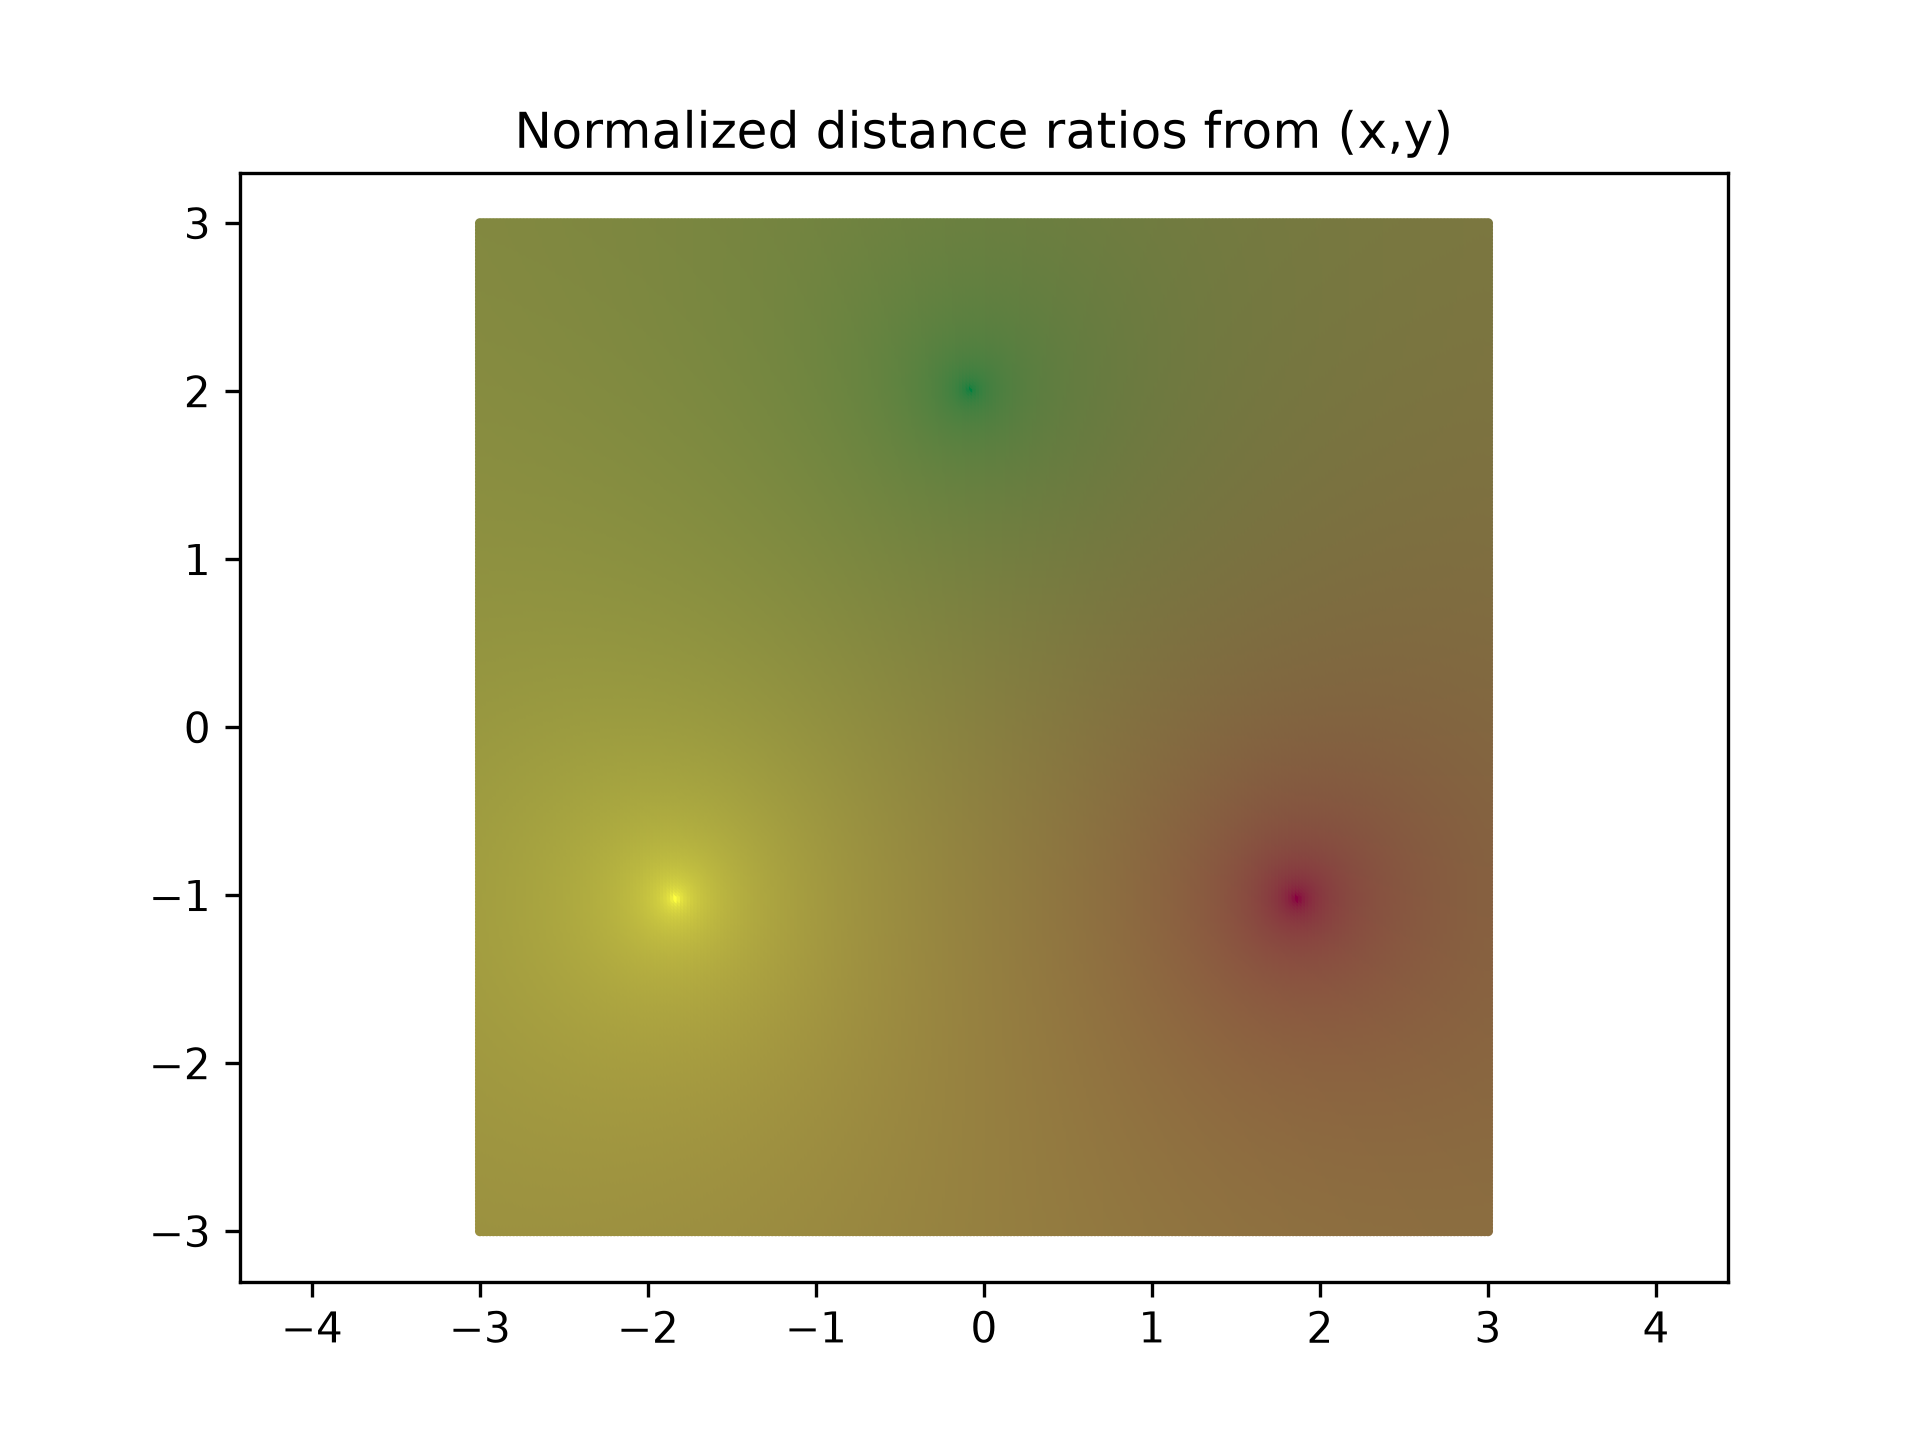
\includegraphics[width=0.5\textwidth]{../code/peripheral/plots/tv ratios.png}
    \caption{Ratios in colour from positions in an example configuration. Ratios have been normalised for better plotting by applying the natural logarithm.}
    \label{fig:2}
\end{figure}

The algorithm might have some problems when both ratios are near \(0.5\) in transposed logarithmic space\footnote{\(\log(1 + r_{ji})\).}, as seen in \autoref{fig:3}, but realistically this just means, that the device is near the first node.

\begin{figure}[h]
    \centering
    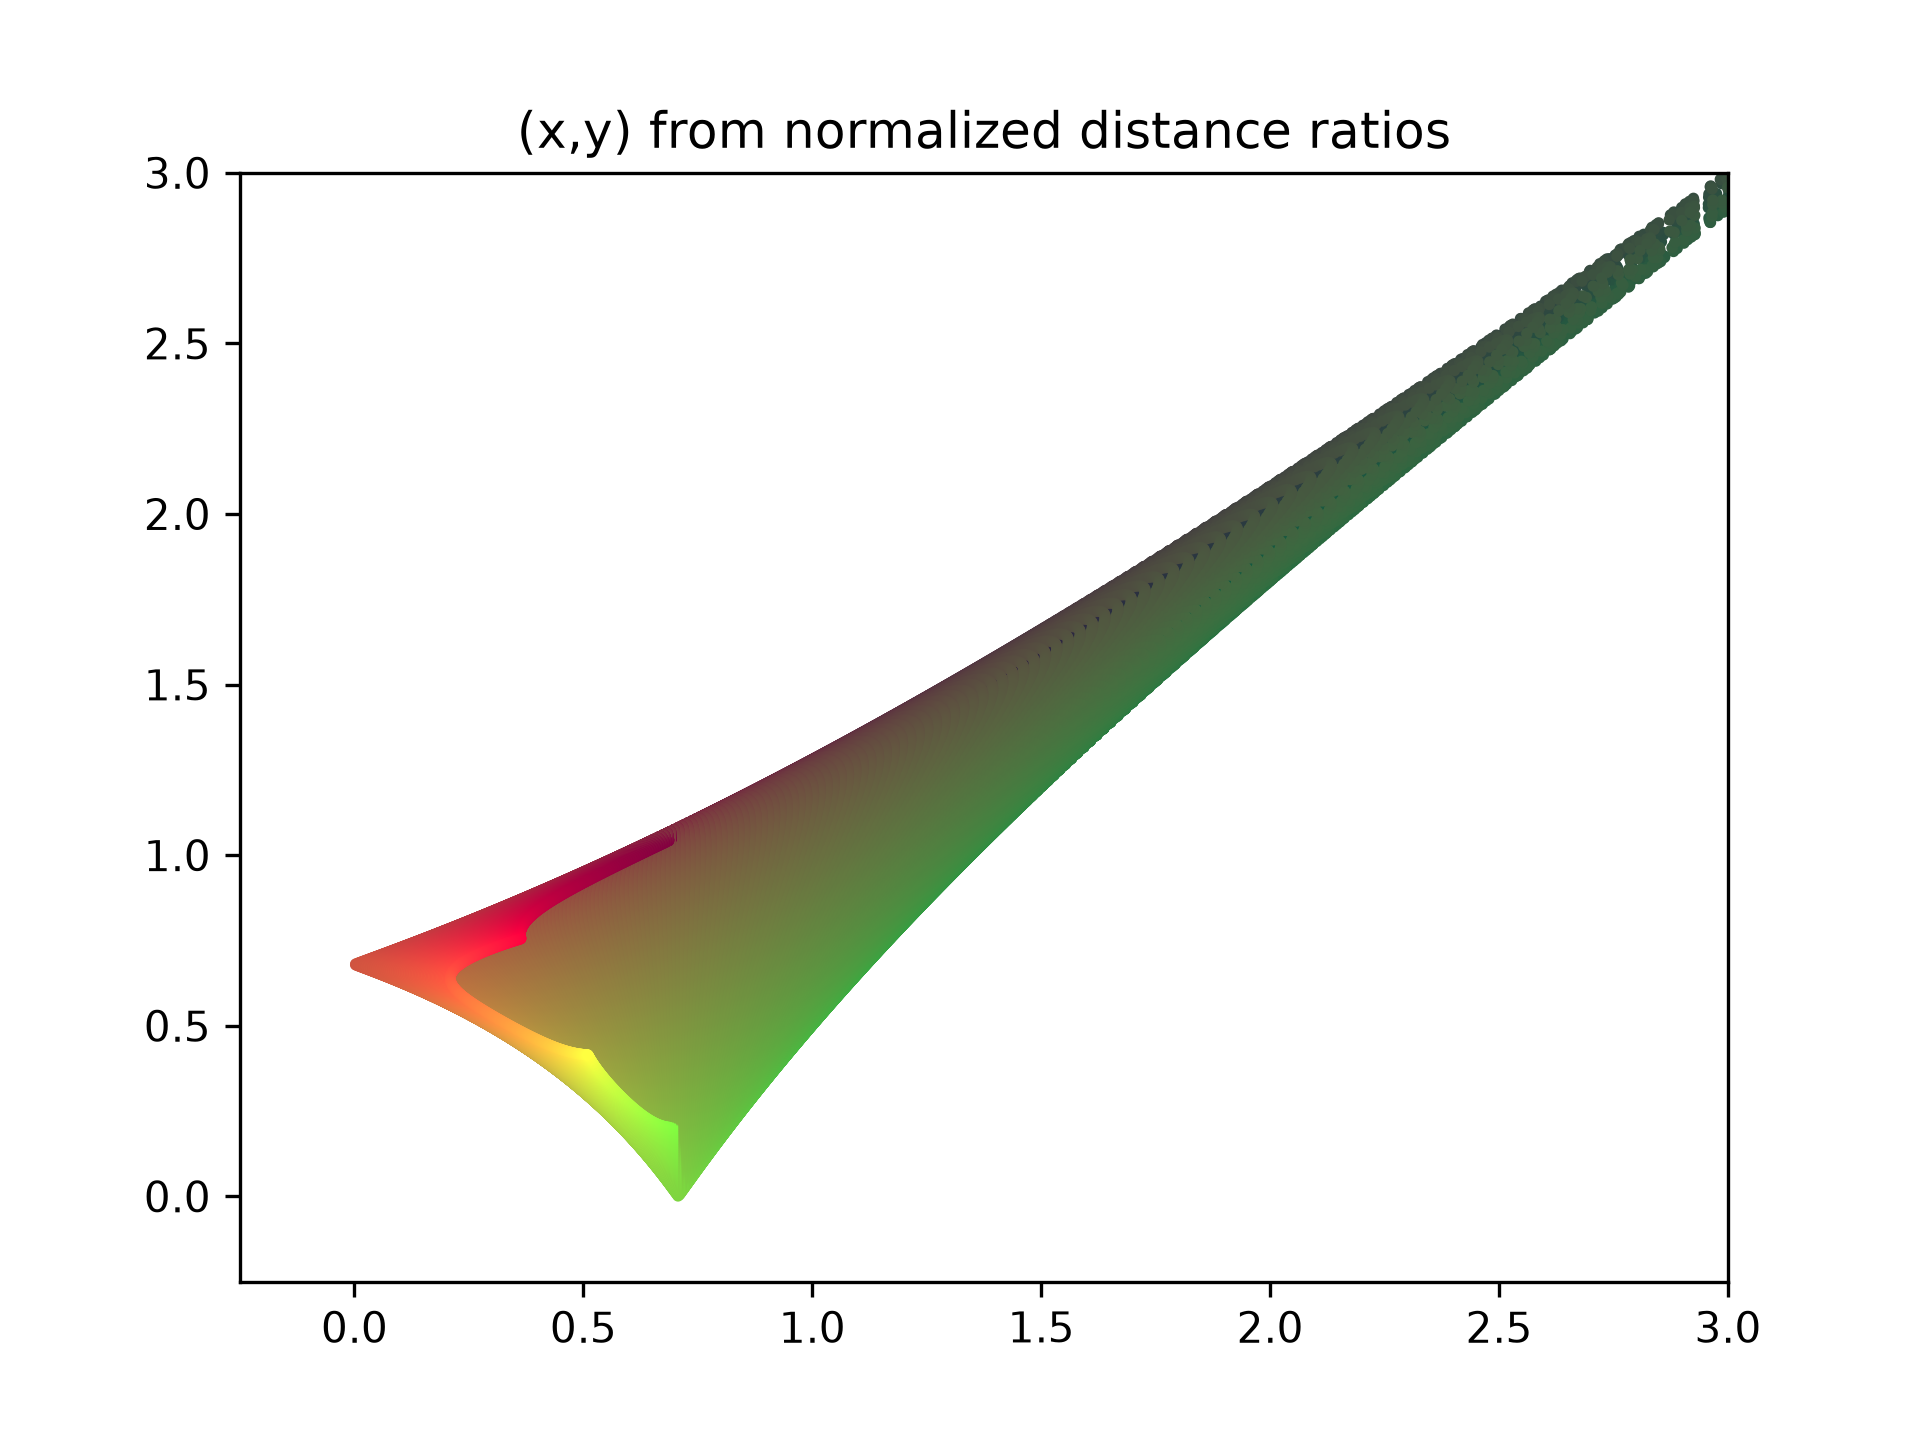
\includegraphics[width=0.5\textwidth]{../code/peripheral/plots/tv xys.png}
    \caption{Positions from normalised ratio space in an example configuration. Ratios have been normalised for better plotting by applying the natural logarithm.}
    \label{fig:3}
\end{figure}

Additionally, the solution works actually pretty good in reality.
Todo: insert video here!
\end{document}
